% Este formato está definido mais acima na seção "APARÊNCIA/FORMATAÇÃO"
\pagestyle{appendix}

% Os apêndices podem ser inseridos diretamente aqui ou "puxados" de outros
% arquivos


\chapter{Tabelas dos demais dados}
\label{ape:tables}

\captionof{table}{Dias com dados faltantes para cada parâmetro de Farinha}
\begin{center}
\begin{tabular}{ c c }
Fe2O3     &   595\\
CaO       &  595\\
SiO2      &   595\\
Al2O3     &   595\\
SO3       &   595\\
P2O5      &   595\\
MgO       &   595\\
K2O       &   595\\
Na2O      &   931\\
CLOR.     &  1697\\
FLUOR.    &  1588\\
FSC       &   595\\
MS        &   595\\
MA        &   595\\
RSA       &   815\\
P. F AL.  &   593 \\
\end{tabular}
\end{center}

\newpage
\captionof{table}{Dias com dados faltantes para cada parâmetro de Cimento Cru}
\begin{center}
\begin{tabular}{ c c }
Alim. (t/h)       & 131\\
Prod (ton)        & 250\\
Calc. (\%)        & 131\\
Arg. (\%)         & 131\\
Areia (\%)        & 132\\
Corr. (\%)        & 370\\
Caulim (\%)       & 421\\
Cinza (\%)        & 295\\
Alurox (\%)       & 442\\
Fe2O3             & 44\\
CaO               & 44\\
SiO2              & 44\\
Al2O3             & 44\\
SO3               & 44\\
P2O5              & 44\\
MgO              &  44\\
K2O              &  44\\
Na2O             &  48\\
MA               &  44\\
MS               &  44\\
FSC              &  44\\
\#100             & 187\\
\#170             &  44\\
Umid Calc (\%)   &  413\\
Umid Arg (\%)    &  414 \\
Umid Areia (\%) &    391 \\
\end{tabular}
\end{center}

\newpage
\captionof{table}{Dias com dados faltantes para cada parâmetro de Clínquer}
\begin{center}
\begin{tabular}{ c c }
 CaOL       &      596\\
Fe2O3       &    596\\
CaO         &   596\\
SiO2        &  596\\
Al2O3       & 596\\
P2O5        & 596\\
MgO         & 596\\
K2O         & 596\\
Na2O        & 596\\
CLOR        & 2724\\
FLUOR       & 2095\\
MS          & 596\\
MA          & 596\\
FSC         & 596\\
RSA         & 809\\
C3S         & 596\\
C2S         & 596\\
C3A         & 596\\
C4AF        & 596\\
F.liq       & 596\\
25,4 mm     & 2753\\
12,7 mm     & 2752\\
6,35  mm    & 2752\\
3,36 mm     & 2752\\
\textless 3,36 mm    & 2756
\end{tabular}
\end{center}

\chapter{Gráficos dos demais índices testados}
\label{ape:graphs}


\begin{figure}[H]
\centering
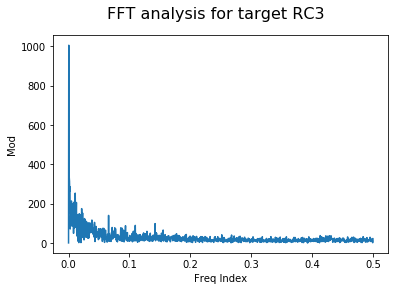
\includegraphics[width=0.9\columnwidth]{FFT_RC3.png}
\caption{Análise Espectral para preditor RC3}
\end{figure}

\begin{figure}[H]
\centering
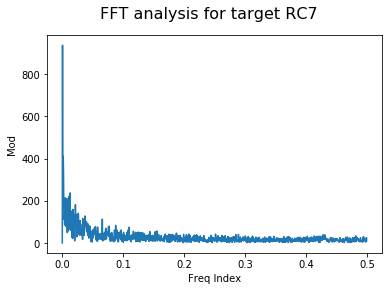
\includegraphics[width=0.9\columnwidth]{FFT_RC7.png}
\caption{Análise Espectral para preditor RC7}
\end{figure}

\begin{figure}[H]
\centering
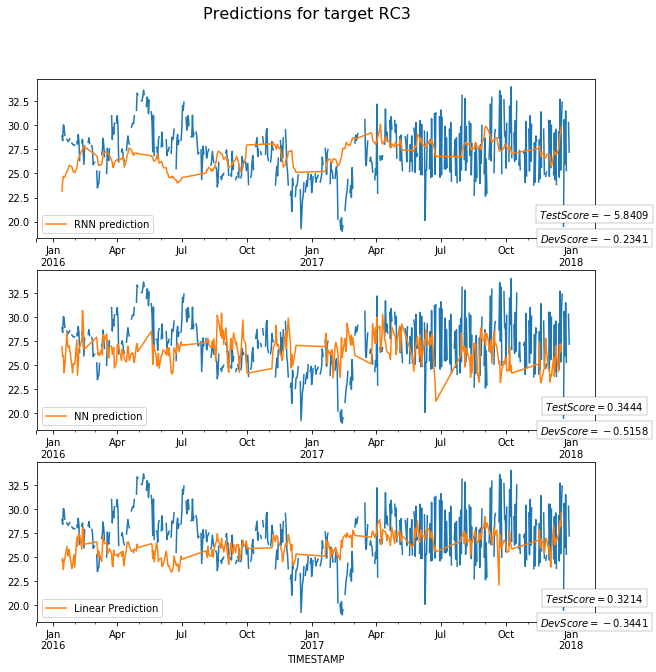
\includegraphics[width=0.9\columnwidth]{RC3.png}
\caption{Comparação dos 3 modelos não-sequenciais na tarefa de regressão do índice RC3}
\end{figure}

\begin{figure}[H]
\centering
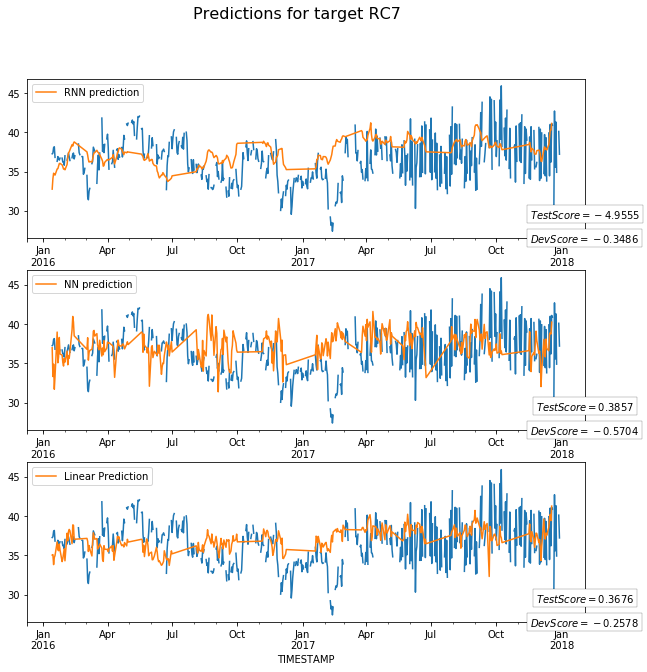
\includegraphics[width=0.9\columnwidth]{RC7.png}
\caption{Comparação dos 3 modelos não-sequenciais na tarefa de regressão do índice RC7}
\end{figure}

\begin{figure}[H]
\centering
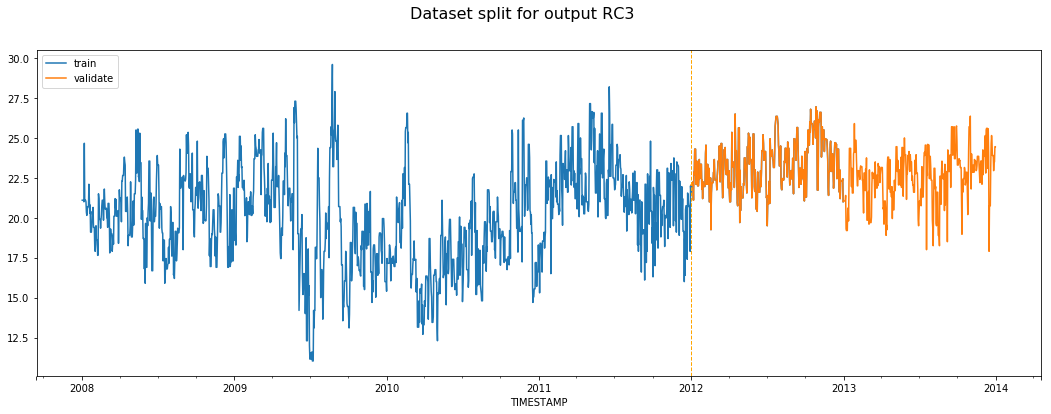
\includegraphics[width=0.9\columnwidth]{dataset_splitRC3.png}
\caption{Divisão do dataset no segundo ensaio para a saída RC3}
\end{figure}

\begin{figure}[H]
\centering
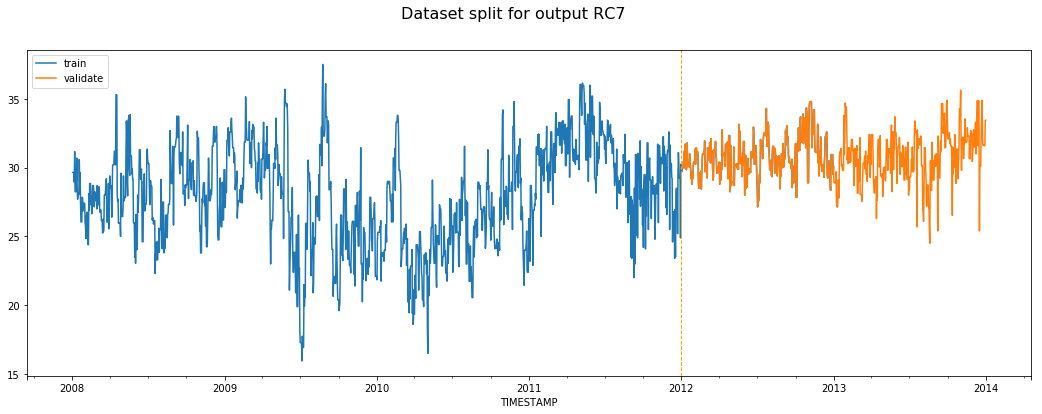
\includegraphics[width=0.9\columnwidth]{dataset_splitRC7.png}
\caption{Divisão do dataset no segundo ensaio para a saída RC7}
\end{figure}

\begin{figure}[H]
\centering
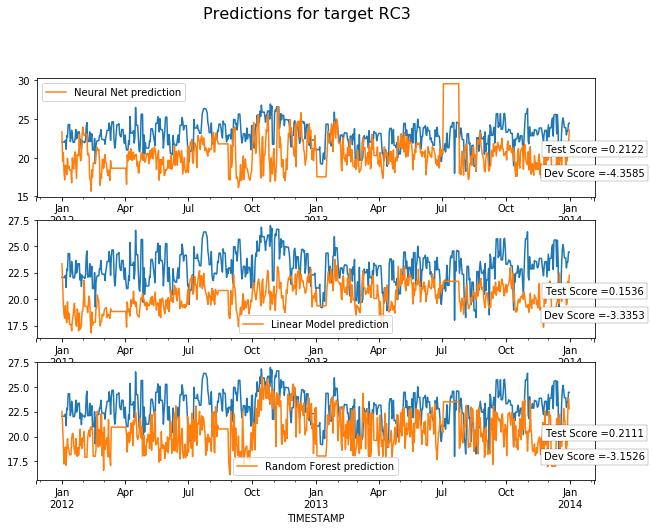
\includegraphics[width=0.9\columnwidth]{farinha_2008-2012-2014RC3.png}
\caption{Comparação dos 3 modelos não-sequenciais na tarefa de regressão do índice RC3}
\end{figure}

\begin{figure}[H]
\centering
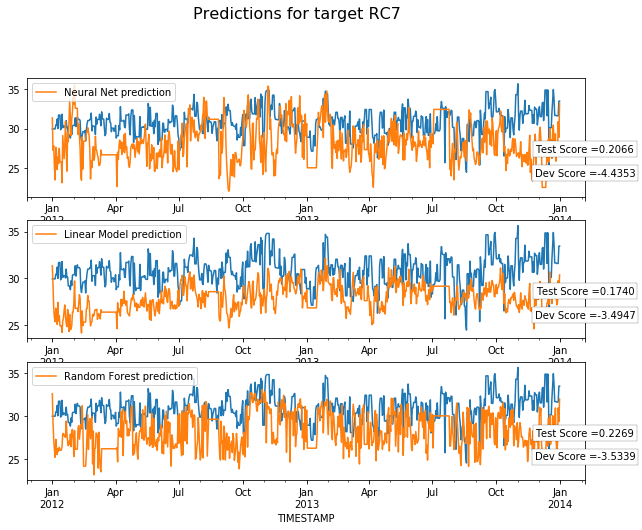
\includegraphics[width=0.9\columnwidth]{farinha_2008-2012-2014RC7.png}
\caption{Comparação dos 3 modelos não-sequenciais na tarefa de regressão do índice RC7}
\end{figure}

